\chapter{合情推理}\label{chap:plausible-reasoning}

1983年,心理学家Amos Tversky和Daniel Kahneman进行了一个著名的实验,他们向一组被试提出了如下问题:Linda是一位单身、外向且年龄为31岁的女性. 在大学期间,她主修哲学,十分关注种族歧视和社会公正问题,而且曾参加过反核游行. 请给下面几个选项发生的可能性排序,1代表最可能,8代表最不可能:
\begin{enumerate}
    \item Linda是一个小学老师.
    \item Linda在书店工作,并且参加瑜伽课程.
    \item Linda非常积极参加女权运动.
    \item Linda是一个精神病的护理员.
    \item Linda是美国女性选民联盟的成员.
    \item Linda是一名银行出纳员.
    \item Linda是一个保险销售员.
    \item Linda是一名银行出纳员,同时她还非常积极参加女权运动.
\end{enumerate}

他们对以下三组人进行了同样的实验:
\begin{enumerate*}[label=(\arabic*)]
    \item 88名来自斯坦福大学或不列颠哥伦比亚大学(UBC)的本科生,没有学过概率统计,
    \item 53名斯坦福大学的一年级研究生,他们学过一门或更多的概率统计课程,
    \item 32名斯坦福大学商学院博士生,他们学过很多概率统计和决策理论的进阶课程.
\end{enumerate*}

我们重点关注第三、六、八个选项. 抽象地来说,我们可以把这三个陈述分别记为$A$, $B$, $A\wedge B$. 从逻辑的角度来看$A\wedge B$发生的时候,$A$和$B$都一定发生,因此$A$(或$B$)更可能发生. 然而,让人大跌眼镜的是,实验结果显示,所有三组人的打分中,超过85\%的人认为$A\wedge B$更可能发生!

以上现象被称为\emph{合取谬误},它表明人类的推理并不等同于我们所理解的逻辑推理(被称为\emph{演绎推理}). 合取谬误的背后隐藏了一种新的推理方式,被称为\emph{合情推理}. 演绎推理很早就有了非常严格的逻辑学框架,得到了充分的研究. 然而,合情推理同样甚至更加重要,它不仅是人类与生俱来的能力,更是科学研究和AI的逻辑基础. 

本章试图建立合情推理的一个数学模型,这一模型与Bayes概率论紧密地联系在一起. 我们会它来研究一些有趣的推理谬误,包括合取谬误,并与演绎推理进行对比. 最后,我们会讨论Bayes概率论中先验为什么是存在的.

\section{命题逻辑的演绎推理}

作为回顾,本节讨论\emph{演绎推理},它最主要的应用场景是数学证明和一些逻辑论证. 演绎推理定义了数学中一些非常重要的概念,例如“公理”“定理”“证明”. 我们会看到,与演绎推理密切相关的是\emph{形式推理系统},它尝试将推理的过程抽象为一堆字符串的变换. 作为介绍,我们这里给出\emph{命题逻辑}的形式推理系统,它是最基本的形式推理系统. 

\emph{命题}是一种陈述,它可以被判定为真或者假. 例如,“北京是中国的首都. ”是一个命题,而“北京是中国的首都吗?”是一个疑问句,所以不是命题. 然而,利用自然语言定义命题,很难判断一些奇怪的句子是不是命题:

\begin{example}
考虑句子$A$:“这句话是假的. ”是一个命题吗?首先,$A$是一个陈述句. 那它的真假呢?
\begin{itemize}
    \item 如果$A$是真的,$A$说的是“这句话是假的”,这与$A$真矛盾,所以它不是真的. 
    \item 如果$A$是假的,$A$的含义是“这句话是真的”,这与$A$假矛盾,所以它不是假的. 
\end{itemize}
因此,这句话既不是真的也不是假的!
\end{example}

以上的现象被称为\emph{自指},也就是一个东西在描述自己.

自指为讨论命题的概念带来了非常大的麻烦. 为了避免这些麻烦,我们回避命题到底是什么这一哲学问题,而是把他们抽象为一些字符串,这就是\emph{命题公式}:

\begin{definition}[命题公式]
\textbf{命题公式}(或简称\textbf{公式})是由一些\textbf{命题变元}和\textbf{连接词}组成的字符串,它们满足以下递归定义:
\begin{itemize}
    \item 命题变元$p,q,r,\dots$是命题公式. 
    \item 如果$\phi$和$\psi$是命题公式,那么$(\neg\phi)$,$(\phi\vee\psi)$,$(\phi\wedge\psi)$,$(\phi\leftrightarrow\psi)$和$(\phi\to\psi)$都是命题公式. 
\end{itemize}

$\neg,\vee,\wedge,\leftrightarrow,\to$被称为\emph{连接词},$\neg$被称为\emph{否定},$\vee$被称为\emph{析取}(\emph{或}),$\wedge$被称为\emph{合取}(\emph{与}),$\leftrightarrow$被称为\emph{双向蕴含}(\emph{等价}),$\to$被称为\emph{蕴含}(\emph{推出}). 在不产生混淆的时候也会省略括号. $A\wedge B$也常写作$AB$,$\neg A$也常写作$\overline{A}$.
\end{definition}

\begin{example}
$(p\vee(q\to r))$是命题公式,但是$p\vee\vee q$不是. 
\end{example}

命题最重要的概念是“真假”,因而命题逻辑一个重要的问题是:\emph{什么样的公式是真的?}给定一个公式集$\Gamma$,对一个公式$\phi$,我们有两种真的概念:
\begin{itemize}
    \item \emph{语义}:$\Gamma\vDash \phi$.
    \item \emph{语形}:$\Gamma\vdash \phi$.
\end{itemize}

首先看语义. 所谓语义,就是“句子的含义”. 在命题逻辑中,句子就是命题公式,而含义就是真假. 既然命题公式是递归定义的,命题公式的真假我们也应该递归定义. 

\begin{definition}[赋值]
给定命题变元集合$V$,它形成的命题公式的集合是$L$,一个\textbf{赋值}是一个从$L$到$\{\T,\F\}$的映射$v$,递归定义如下:
\begin{itemize}
    \item 如果$\phi=p\in V$,那么$v(\phi)=v_p$.
    \item 如果$\phi=\neg\psi$,那么$v(\phi)=\begin{cases} \T, & v(\psi)=\F, \\ \F, & v(\psi)=\T. \end{cases}$
    \item 如果$\phi=\psi\vee\chi$,那么$v(\phi)=\begin{cases} \T, & v(\psi)=\T\text{ 或}~v(\chi)=\T, \\ \F, & v(\psi)=\F\text{ 且}~v(\chi)=\F. \end{cases}$
    \item 如果$\phi=\psi\wedge\chi$,那么$v(\phi)=\begin{cases} \T, & v(\psi)=\T\text{ 且}~v(\chi)=\T \\ \F, & v(\psi)=\F\text{ 或}~v(\chi)=\F. \end{cases}$
    \item 如果$\phi=\psi\to\chi$,那么$v(\phi)=\begin{cases} \T, & v(\psi)=\F\text{ 或}~v(\chi)=\T, \\ \F, & v(\psi)=\T\text{ 且}~v(\chi)=\F. \end{cases}$
    \item 如果$\phi=\psi\leftrightarrow\chi$,那么$v(\phi)=\begin{cases} \T, & v(\psi)=v(\chi), \\ \F, & v(\psi)\neq v(\chi). \end{cases}$
\end{itemize}
\end{definition}

以上定义看起来比较冗长,但是符合我们的直觉. 一种更为直观的表达方式是\emph{真值表}. 注意,连接词可以被理解为一个真值向量到真值的映射,例如$\wedge$可以被理解为$\{\T,\F\}^2\to\{\T,\F\}$的映射,这一映射可以用真值表表示:

\begin{center}
\begin{tabular}{cc|c}
    $p$ & $q$ & $p\wedge q$ \\
    \hline
    $\T$ & $\T$ & $\T$ \\
    $\T$ & $\F$ & $\F$ \\
    $\F$ & $\T$ & $\F$ \\
    $\F$ & $\F$ & $\F$ \\
\end{tabular}
\end{center}
于是,定义中的递归可以用直接用$\wedge$来表示:如果$\phi=\psi\wedge\chi$,那么$v(\phi)=v(\psi)\wedge v(\chi)$.

我们看一个例子. 

\begin{example}
考虑公式$(p\wedge q)\to r$,我们来定义赋值$v$. 首先给命题变元赋值:
\[\begin{array}{c|ccc}
    &p&q&r\\\hline
    v&\F&\T&\F\\
\end{array}\]
然后递归计算公式的真值. 首先计算$(p\wedge q)$的真值. 根据真值表,我们有
\[v(p\wedge q)=v(p)\wedge v(q)=\F\wedge\T=\F.\]
然后计算$(p\wedge q)\to r$的真值:
\[v((p\wedge q)\to r)=v(p\wedge q)\to v(r)=\F\to\F=\T.\]
\end{example}

接下来,我们从赋值到推理. 推理是从\emph{前提}出发,得到\emph{结论}的过程. 和赋值相关的推理概念有如下定义:

\begin{definition}[语义蕴含]
给定公式集$\Gamma$和公式$\phi$,如果对任意赋值$v$,如果$v(\psi)=\T$对任意$\psi\in\Gamma$都成立,那么$v(\phi)=\T$,则称$\Gamma$\textbf{语义蕴含}$\phi$,记作$\Gamma\vDash\phi$.
\end{definition}

换言之,给定一个真的前提$\Gamma$,我们所关注的公式$\phi$也是真的. 这一概念只关心真值之间的关系,但是至于$\Gamma$如何导致$\phi$为真,不是这一概念可以刻画的. 

\begin{example}\label{ex:semantic-implication}
如果$\Gamma=\{p\to q,q\to r\}$,那么$\Gamma\vDash p\to r$. 我们来证明这个,对任意赋值$v$,如果$v(p\to q)=\T$,那么$v(p)=\F$或者$v(q)=\T$,
\begin{itemize}
    \item 如果$v(p)=\F$,那么$v(p\to r)=\T$.
    \item 如果$v(q)=\T$,那么$v(q\to r)=v(r)$. 因为$v(q\to r)=\T$,所以根据定义$v(r)=\T$,于是$v(p\to r)=\T$.
\end{itemize}
不论在何种情况,都有$v(p\to r)=\T$,即$\Gamma\vDash p\to r$.
\end{example}

接下来,我们看语形. 语形就是“句子的形态“,或者说一个句子是如何构造出来的. 它更像我们所理解的“推理”,也就是从一些公式出发,得出另一些公式. \emph{推导规则}描述了从一些公式出发如何得到另外公式. 语法推导的形式是
\[\begin{array}{c}
        \phi_1\quad\phi_2\quad\dots\quad\phi_n  \\\hline
        \psi
\end{array}\]
横线上方的称为\emph{前提},横线下方的称为\emph{结论}. 

在一些命题逻辑的形式推理系统(比如Hilbert推理系统)中,推导规则只有\emph{一条},即\emph{肯定前件}(MP):
\[\begin{array}{c}
        \phi\to\psi\quad\phi  \\\hline
        \psi
\end{array}\]

然而,引入更多推导规则可以有助于简化推理的过程,这是另外一些形式推理系统(比如自然演绎系统)的做法. 比如,我们可以加入合取和析取的推导规则:
\begin{itemize}
    \item 引入新的连接词,例如
    \[\begin{array}{c}
         \phi\quad\psi  \\\hline
         \phi\wedge\psi
    \end{array}\]
    \item 消除连接词,例如
    \[\begin{array}{c}
        \phi\wedge\psi  \\\hline
        \phi
   \end{array}\]
\end{itemize}
    
我们再看一个非常重要的例子. 

\begin{example}
将\emph{归谬法}(RAA)加入推导法则:将$\neg\phi$作为前提,得到了结论$\F$,那么可以推出$\phi$才是结论. 写作
    \[\begin{array}{c}
         [\neg\phi]  \\
         \vdots\\
         \F\\\hline
         \phi
    \end{array}\]

方括号表示\emph{假设}$[\neg\phi]$是前提,省略号表示推导的中间步骤. 注意,这里是\emph{假设}了一个前提,而不是真的前提,这一点是非常重要的. 利用这一推导规则,我们就可以得到反证法. 
\end{example}


演绎推理所对应的数学模型即为\emph{形式推理系统}:一系列字符串的集合(命题公式),以及一系列的推导规则,以及公理的集合(一些命题公式). 

在形式推理系统中,我们可以形式地定义什么是“推理”和“结论”,而这些东西构成了\emph{演绎推理}的过程与结果:

\begin{definition}[演绎推理]
设$L$是公式集,$A\subseteq L$ 是公理的集合,$\mathcal R$是推导规则,$\Gamma\subseteq L$,考虑$L$中的序列$\phi_1,\dots,\phi_n$,如果对任意$i$,$\phi_i$满足下面的其中一个条件:
\begin{enumerate}
    \item $\phi_i\in A$,
    \item $\phi_i\in\Gamma$,或者
    \item 存在一个推导规则,和$\phi_{i_1},\dots,\phi_{i_k}$,$i_1,\dots,i_k<i$使得$\phi_i$可以由$\phi_{i_1},\dots,\phi_{i_k}$推导出来,
\end{enumerate}
那么称$\phi_1,\dots,\phi_n$是从$\Gamma$出发的一个\textbf{演绎推理},记作$\Gamma\vdash\phi_n$,$\phi_n$称为\textbf{结论},$\Gamma$称为\textbf{前提}.
\end{definition}


简而言之,记号$\Gamma\vdash\phi$的意思是以$\Gamma$作为前提,依据推导法则,通过一系列(但有限)的推理步骤,可以得到$\phi$作为结论. 因而,语形定义的真值是“可以被推理出来”的概念. 对比语义,语形更加关注“过程”,而不是“关系”.

介绍完了语义和语形,我们现在来看他们之间的关系,其中最重要的是\emph{完备性定理}:
\begin{theorem}[完备性定理]
对任意公式集$\Gamma$和任意公式$\phi$,
\[\Gamma\vDash\phi\iff\Gamma\vdash\phi.\]
\end{theorem}

完备性定理有两层意思:能推理出来的都是真的,真的都能被推理出来. 并非所有的形式推理系统都有完备性定理,但是对于命题逻辑来说,这个定理成立的形式推理系统是更加符合直观的. 

完备性定理的一个直接推论是,我们可以用真值表来检查从前提出发是否能推出结论. 例如,在\Cref{ex:semantic-implication} 中我们验证了$p\to q,q\to r\vDash p\to r$\footnote{在书写时,我们常常省略$\Gamma$中的花括号,因此这里写作$p\to q,q\to r\vDash p\to r$而不是$\{p\to q,q\to r\}\vDash p\to r$. 对于符号$\vdash$我们遵循同样的规则.},所以也有
\[p\to q,q\to r\vdash p\to r,\]
即便我们完全不知道这一推理是如何进行的,我们依然知道这一推理是可行的!

如果$\varnothing\vDash \phi$,那么称$\phi$为\emph{重言式}. 重言式是不需要加任何假设也一定成立的公式,是这一推理系统所包含的“正确的废话”. 如果$\psi\leftrightarrow\phi$是重言式,我们就说$\psi,\phi$是\emph{等值}的. 等值的公式在演绎推理中可以互相替代使用. 例如:$p\to q$与$\neg q\to\neg p$是等值的,所以证明一个命题也可以去证明它的逆否命题.


\section{合情推理的数学模型}

现在,我们将话题转到合情推理. 出乎意料的是,人类先天所具备的推理能力,更接近\emph{合情推理}而不是演绎推理. 在婴儿时期,我们需要建立各式各样的经验规则,以便在这个世界生存下来. 例如,如果婴儿碰到了带电的插座,那么他/她会感受到疼痛,这样就知道了插座是危险的. 下次遇到插座的时候,他/她就会避开插座,因为他/她学到了“所有插座都是危险的”这一经验. 上面的例子都是从一些特殊的事件(摸插座触电了)出发,得到了一些一般的结论(所有插座都是危险的),这就是合情推理的基本形式.

为了从更抽象的角度理解合情推理的形式,我们用经典的\emph{三段论}来对比演绎推理和合情推理. 

演绎推理包含两个\emph{强三段论}:
    \[
        \begin{array}{c}
            \begin{array}{c}  
                \phi \to \psi \\ \phi\text{ 是真的} \\ \hline \psi\text{ 是真的}
            \end{array} 
            \qquad \qquad 
            \begin{array}{c}  
                \phi \to \psi \\ \psi\text{ 是假的} \\ \hline \phi\text{ 是假的}
            \end{array}
        \end{array} 
    \]

例如,从科学的角度,触电会疼痛($\phi\to \psi$),摸插座会触电($\phi$),所以摸插座会疼痛($\psi$). 这是一个演绎推理的例子.

然而,合情推理是完全发过来的,即\emph{弱三段论},形式上写作 
        \[
        \begin{array}{c}
            \begin{array}{c}  
                \phi \to \psi \\ \psi\text{ 是真的} \\ \hline \phi\text{ 变得更合理}
            \end{array} 
        \end{array} 
    \]

例如,触电会疼痛($\phi\to \psi$),摸插座会疼痛($\psi$),所以摸插座很可能会触电($\phi$).  这样的推理更符合上面婴儿推理的模式. 虽然我们不能得知$\phi$的真假,但是根据已有的事实$\psi$,我们可以得到$\phi$的合理性推断. 这样没有严格真假的推理模式就是\emph{合情推理}.

推理的一个重要概念是“真假”,或者说这个推理的正确性、合理性. 在演绎推理中,推理只有两种可能:正确的推理和错误的推理;而在合情推理中,推理的合理性有多种可能,例如“很可能正确”“可能正确”“很可能错误”等. 我们来看一个例子. 

\begin{example}
    假如婴儿摸了插座,并且感到了疼痛,那么,你觉得他/她会怎么想?
    \begin{itemize}
        \item 选项1:摸插座是危险的. 
        \item 选项2:摸的插座上面有微小不可见的细针,细针扎了他/她的手指. 
    \end{itemize}
\end{example}
虽然选项1和选项2都是可能的,但是他们的合理程度并不同:选项1明显比选项2要合理得多. 这里产生了一个自然的问题:如何刻画不同推理的合理程度?

\subsection{合情推理的基本假设,似然}

接下来,我们给合情推理建立一个数学模型. 合情推理的基本方式是给定已知的命题$B$,推出命题$A$的\emph{合理程度},比如“非常可能是真的”“可能是真的”“可能是假的”“非常可能是假的”等,我们用符号$A|B$表示这一合理程度. 

在写出符号的时候,我们已经假设了合理程度所对应的数学对象:$A|B$应该是$L\times L\to\R$的函数,这里$L$是命题公式的集合. 但是,这一表述是有瑕疵的,因为不是所有的前提到结论的推理都可以用合理程度来描述. 比如,$B$是“太阳从西边升起“,前提根本就是一个假命题,从假命题出发,何谈“合情”?所以,符号$A|B$应该只对一些特定的$A,B$有意义,我们称之为$L\times L\to\R$的\emph{偏函数},并将这一函数写为$f(A|B)$,称作\emph{似然}.

我们还没有确定这一映射的具体形式. 但是,这样的映射要满足两个原则:
\begin{enumerate*}
    \item 符合我们对于合情推理的基本直观,
    \item 易于计算.
\end{enumerate*}

在这里,我们类比行星运动定律来理解这第二个原则的具体含义. 最开始的时候,人们认为天体都是绕着地球转的. 基于这样的思想,Ptolemaeus提出了行星运动的模型. 在这个模型中,Ptolemaeus引入了“均轮”和“本轮”的概念. 行星在一个较小的圆(本轮)上做匀速圆周运动,而这个本轮的中心又在一个更大的圆(均轮)上绕地球做匀速圆周运动. 这一模型可以较为准确预测天体的运动,然而需要非常复杂的概念. 

后来,Kepler提出了完全不同的行星运动模型:行星绕着恒星做椭圆运动,与恒星的连线扫过的面积与运动时间成正比,行星轨道的半长轴的三次方与其公转周期的二次方的比值都相等. 这就是著名的“Kepler三定律”. 在Kepler的模型中,我们放弃了“均轮”和“本轮”的概念,而是用简单的椭圆来描述行星的运动. 尽管Ptolemaeus模型和Kepler模型都可以描述行星的运动,但是Kepler模型更加简单,更加容易计算,也正是在此基础上,Newton才发现了万有引力定律. 

同样的道理也适用于合情推理. 或许会有很多的$f$可以符合直观地描述合理程度,但是我们希望找到一个尽可能容易使用和计算的$f$,它能有更广泛的应用,或许也蕴含了更深层次的规律. 现在,我们暂时将所有符合合情推理直观的映射的集合记作$\mathcal L$. 我们给出$\mathcal L$中的函数要具备的性质(即假设),然后再确定具体的函数. 

首先,在命题逻辑中,我们只关心命题的真假,并不关心命题具体是什么. 在合情推理中,我们依然希望有这样的性质:推理的合理程度不依赖具体的命题形式. 在数学上,这等价于如下的原则:

\begin{principle}[等值原则]
    对任意$f\in\mathcal L$,任意命题公式$\phi_1,\phi_2,\psi\in L$,如果$\phi_1$和$\phi_2$等值(即$\phi_1\leftrightarrow\phi_2$是重言式),那么
    \[
        f(\phi_1|\psi)=f(\phi_2|\psi).
    \]
\end{principle}

例如,$\phi\to \psi$和$\neg \phi\vee \psi$的具体含义是不同的:一个是蕴含式(即$\phi$推出$\psi$),一个是两个命题($\neg \phi$和$\psi$)的或;但是他们等值,所以$f(\phi\to \psi | \xi)=f(\neg \phi\vee \psi|\xi)$. 更多的例子如下:

\begin{example}
    对任意$f\in\mathcal L$以及公式$\alpha,\beta,\gamma$,成立
    \begin{itemize}
        \item $f(\alpha\vee \beta | \gamma)=f((\beta\vee \alpha) | \gamma)$.
        \item $f((\alpha\beta)\gamma|\delta)=f(\alpha(\beta\gamma)|\delta)$.
        \item $f(\neg\neg \alpha|\beta)=f(\alpha|\beta)$.
    \end{itemize}
\end{example}

现在我们来看第二条假设,它与推理不同的路径有关. 考虑从$\gamma$出发推出$\alpha\beta$为真. 我们有两种推理的链条:
\begin{enumerate}
    \item 直接推理:直接从$\gamma$推出$\alpha\beta$.
    \item 分步推理:先从$\gamma$推出$\alpha$,然后从$\alpha\gamma$推出$\beta$,因此自然也推出了$\alpha\beta$.
\end{enumerate}
也可以用下面的图来直观表示,其中实线箭头表示直接推理,虚线箭头表示分步推理:

\begin{center}
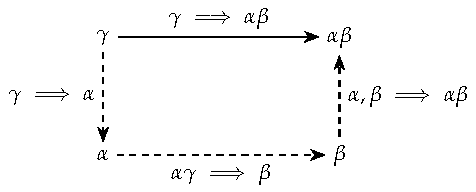
\includegraphics{Figures/plausible-reasoning/two-chain-reasoning.pdf}
\end{center}

我们前面要求,“推理的合理程度不依赖具体的命题形式”,现在,我们将这一要求进一步细化为“推理的合理程度不依赖推理的具体形式”. 因为上面的直接推理和分步推理都是从$\gamma$推出$\alpha\beta$,所以我们要求他们的合理程度相同,即

\begin{hypothesis}
    对任意$f\in\mathcal L$,存在一个$\R\times\R\to\R$的函数$F$,对任意命题公式$\alpha,\beta,\gamma$,
    \[
        f(\alpha\beta|\gamma)=F(f(\alpha|\gamma),f(\beta|\alpha\gamma)).
    \]
\end{hypothesis}

换言之,在考虑我们不关心$\gamma$具体是怎么推出来$\alpha$的,我们只要求$\alpha\beta$的合理程度与$\alpha$和$\beta$的合理程度有关. 

注意,以上假设不能写成$f(\alpha\beta|\gamma) = F(f(\beta|\gamma), f(\alpha|\gamma))$. 例如,假设$\alpha$是“小明的左眼是蓝色的”,$\beta$是“小明的右眼是棕色的”. $f(\alpha|\gamma)$和$f(\beta|\gamma)$都可以很合理,但$f(\alpha\beta|\gamma)$则非常罕见. 同样的道理,我们可以排除其他形式的假设,比如$f(\alpha\beta|\gamma) = F(f(\gamma|\alpha), f(\beta|\gamma))$.

我们定义的$F$具有如下性质:
\begin{theorem}
    如果$F$是二阶连续可微函数,那么$F$充分必要地满足
        \[cf(F(p,q))=f(p)f(q),\]
        这里,$c$是某个常数,$f$是某个函数.
        因此,对任意命题公式$\alpha,\beta,\gamma$,成立
        \[cf(\alpha\beta|\gamma)=f(\alpha|\gamma)f(\beta|\alpha\gamma).\]
    \end{theorem}

回忆,我们的目标是找到一个尽可能简单的$f$,它能够描述合情推理的合理程度. 因此,我们可以接受$F$二阶连续可微的假设,然后让$c=1$. 于是,我们得到了合情推理的一个基本原则:
\begin{principle}[与规则]
对命题$\alpha,\beta,\gamma$,成立
\[f(\alpha\beta|\gamma)=f(\alpha|\gamma)f(\beta|\alpha\gamma).\]
\end{principle}

第二个考虑的是似然$f(\alpha|\beta)$和$f(\neg\alpha|\beta)$的关系. 两个似然应该存在某种函数关系,于是我们有如下假设:

\begin{hypothesis}
    对任意$f\in\mathcal L$,存在函数$S:\R\to\R$,对任意命题公式$\alpha,\beta$,成立
    \[f(\neg\alpha|\beta)=S(f(\alpha|\beta)).\]
\end{hypothesis}

在与规则限制之下,我们可以证明$S$具有如下性质:
\begin{theorem}
    如果$S$二阶连续可微,那么$S$充分必要地满足
    \begin{equation*}
        S(x) = (1 - x^m)^{1/m},
    \end{equation*}
    这里的$m$是一个正常数.
\end{theorem}

由上面的定理,我们可以得到以下性质
\begin{corollary}
    $f(\alpha|\beta)^m + f(\neg\alpha|\beta)^m = 1$.
\end{corollary}
\begin{proof}
    $f(\neg\alpha|\beta) = S(f(\alpha|\beta)) = (1 - f(\alpha|\beta)^m)^{1/m}$.
\end{proof}

同样,从简洁性的角度出发,我们可以接受$S$二阶连续可微的假设,然后让$m=1$. 于是,我们得到了合情推理的另一个基本原则:
\begin{principle}[否定规则]
对命题$\alpha,\beta$,成立
\[f(\alpha|\beta) + f(\neg\alpha|\beta) = 1.\]
\end{principle}

由上,我们得到了合情推理的三个基本原则:等值原则、与规则和否定规则. 这三个原则构成了合情推理的基本框架.

接下来,我们说明,这三个原则就已经足够用来计算任意的合情推理. 首先,连接词$\{\wedge,\neg\}$组成了演绎逻辑的完备集:所有真值函数都可以用这个集合的词来表示,因此,根据等值规则,只要可以计算包含$\wedge$和$\neg$的合情推理,就可以计算任意合情推理. 其次,我们可以用与规则和否定规则来计算$\wedge$,否定规则计算$\neg$,因此,任何命题都可以通过这三个原则来计算.

\begin{example}
    例如,计算$f(A\vee B|C)$,
        \begin{align*}
            f(A \vee B|C) 
            &= 1 - f(\overline{A}\wedge\overline{B}|C)\\
            & = 1 - f(\overline{A}|C)f(\overline{B}|\overline{A}C) \\
            &= 1 - f(\overline{A}|C)(1 - f(B|\overline{A}C))\\
            &= f(A|C) + f(\overline{A}B|C) \\
            &= f(A|C) + f(B|C)f(\overline{A}|BC) \\
            &= f(A|C) + f(B|C)(1 - f(A|BC))\\
            &= f(A|C) + f(B|C) - f(AB|C).
        \end{align*}
\end{example}


\subsection{似然与概率}
我们已经知道,似然是一个合理性度量,在本节中,我们将似然与概率联系起来:他们实际上是等价的.

首先介绍\emph{Kolmogorov}的概率论,详细的讨论见\Cref{chap:prob}. 这一概率论研究事件空间上的概率测度. 其研究对象的总体被称为\emph{样本空间},记为$\Omega$. 我们只能观测到某种可观测的特性$P$,而不能直接观测样本点,即我们只能观察\emph{事件},或者说集合
    \[\{\omega\in \Omega:P(\omega)\}.\]
我们可以观测的所有事件的集合称为\emph{事件域},记为$\mathscr{F}$.

事件域$\mathscr{F}$中的事件之间互相有关联. 我们自然可以观测到$\Omega$,因此$\Omega\in\mathscr{F}$. 如果我们可以观测到事件$A$,那么我们也可以通过没有观测到$A$来判断观测到了$\Omega\setminus A$. 因此,$A\in\mathscr{F}\implies \Omega\setminus A\in\mathscr{F}$. 如果我们观测到了$A$或者$B$,我们其实也观测到了$A\cup B$,即$A,B\in\mathscr{F}\implies A\cup B\in\mathscr{F}$.

事实上,我们可以形式上定义概率:
\begin{definition}[概率]
\textbf{概率}$\Pr$是一个事件域$\mathscr{F}$到实数的映射,并且满足:
    \begin{itemize}
        \item 规范性:$\Pr(\Omega)=1$.
        \item 非负性:对任意$A\in\mathscr{F}$,$\Pr(A)\in[0,1]$.
        \item 可列可加性:对$A_1,A_2,\dots$满足$A_i\cap A_j=\varnothing,i\neq j$,有
        \[\Pr\left(\bigcup_i A_i\right)=\sum_i \Pr(A_i).\]
    \end{itemize}
\end{definition}

事件是命题的集合论描述. 具体来说,有如下对应
    \[\begin{array}{c|c}
         \text{事件}&\text{命题}  \\\hline
         \Omega & \T\\
         \varnothing & \F\\
         A\cap B& A\wedge B\\
         A\cup B& A\vee B\\
         A\subseteq B& A\to B\\
         A=B&A\leftrightarrow B
    \end{array}\]

回忆条件概率的定义,我们可以得到链式法则:
    \[\Pr(AB|C)=\frac{\Pr(ABC)}{\Pr(C)}=\frac{\Pr(B|AC)\Pr(AC)}{\Pr(C)}=\Pr(B|AC)\Pr(A|C).\]
回忆补事件公式:$\Pr(A|C)+\Pr(\overline{A}|C)=\Pr(\Omega|C)=1$. 这两个公式恰好对应了合情推理的与规则以及否定规则!

这并不是巧合,实际上,合情推理与事件域的公理化概率具有一一对应的关系,见\Cref{tab:prob}.
    \begin{table}[ht]
        \centering
        \begin{tabular}{c|c}
        公理化概率论&合情推理  \\\hline
        事件 & 命题\\
        (条件)概率 & 似然\\
        链式法则 & 与规则\\
        补事件公式 & 否定规则
        \end{tabular}
        \caption{概率论与合情推理的对应}
        \label{tab:prob}
    \end{table}

从这个意义上说,概率是似然唯一的数学模型!从此,我们将似然$f(A|B)$定义为概率$\Pr(A|B)$.

\subsection{先验与基率谬误}

在前面,我们有意模糊了条件概率和概率在合情推理中的区别. 然而,这样的区别是非常重要的. 在合情推理中,非条件的概率被称为\emph{先验概率}或者\emph{基率},它表示了对这个命题合理程度的一种无条件的信念. 对应地,条件概率就是\emph{后验概率}或\emph{似然},它表示了对合情推理合理程度的一种信念.先验概率和后验概率有若干相互转化的公式.

条件概率有全概率公式:
\begin{theorem}[全概率公式]
设$A_i$是彼此互斥的事件,$\cup_i A_i=\Omega$,那么
    \[\Pr(B)=\sum_{i}\Pr(B|A_i)\Pr(A_i).\]
\end{theorem}
全概率公式表明了如何使用似然建立起不同先验概率之间的联系.

条件概率还有Bayes定理:
\begin{theorem}[Bayes定理]
    \[\Pr(A|B) = \Pr(B|A)\frac{\Pr(A)}{\Pr(B)}.\]
\end{theorem}
 Bayes定理表明了两个不同的后验概率如何基于先验概率相互转化. 在合情推理中,这表明了前提推结果的强三段论和结果推前提合理性的弱三段论之间的关系.

 下面我们看一个合情推理的例子. 一辆出租车在夜间发生了一起肇事逃逸事故. 这座城市有两家出租车公司,绿色和蓝色. 这个城市历史上肇事逃逸车辆85\%是绿色的,15\%是蓝色的. 一名目击者指认出租车是蓝色的,这里的指认并不一定正确. 考虑一种理想的假设,法庭知道这位证人80\%的概率能正确识别颜色,20\%的概率会把颜色识别错.问:事故车辆是那种颜色的可能性更大?忽略先验概率会产生答案是蓝车的结论.

下面我们考虑先验概率再次做计算. 记 $B$ 为肇事逃逸的出租车为蓝色,$G$ 为肇事逃逸的出租车为绿色,$R$为目击者指认出租车是蓝色. 先验概率为$\Pr(B) = 0.15$,$\Pr(G) = 0.85$. 似然为$\Pr(R|B) = 0.8$, $\Pr(R|G) = 0.2$. 利用全概率公式,$\Pr(R) = \Pr(B)\Pr(R|B) + \Pr(G)\Pr(R|G)  =0.29$. 

利用Bayes定理,$\Pr(B|R) = \Pr(R|B){\Pr(B)}/{\Pr(R)}\approx 0.41$. 然而,$\Pr(G|R) = \Pr(R|G){\Pr(G)}/{\Pr(R)}\approx 0.59$. 因此我们更应该倾向于认为肇事逃逸的出租车是绿色的!

上面的例子表明人类决策有一种忽略先验概率的倾向,这种倾向被称为\emph{基率谬误}. 为了研究这种谬误,我们将先验概率也纳入合情推理的模型之中. 这样,Kolmogorov的概率论和合情推理就完全一致了. 反过来说,如果我们将概率论理解为如上合情推理的数学模型,我们就得到了\emph{Bayes概率论}.

\section{合情推理的归纳强论证}

\subsection{归纳强论证}

在基率谬误的例子中,我们看到合情推理必须要完整地考虑先验的影响.另一方面,我们看到最终做出决策的方式是\emph{最大似然},即似然更高的那个命题更有可能是对的. 这说明合情推理中有很不同于演绎推理的论证方式.

我们首先指出合情推理包含了命题逻辑中的两个强三段论:
        \[
        \begin{array}{c}
            \begin{array}{c}  
                A \to B \\ A\text{ 是真的} \\ \hline B\text{ 是真的}
            \end{array} 
            \qquad \qquad 
            \begin{array}{c}  
                A \to B \\ B\text{ 是假的} \\ \hline A\text{ 是假的}
            \end{array}
        \end{array} 
    \]
我们以第一个三段论为例,记$C \equiv A \to B$. 由链式法则,$\Pr(B|AC) = \Pr(AB|C) / \Pr(A|C)$. $A \to B$意味着作为事件$A\subseteq B$,即$AB=A$,$\Pr(AB|C) = \Pr(A|C)$. 代入上式得到 $\Pr(B|AC) = 1$,这就是说,当$A$为真时,$B$也为真.

除了演绎逻辑中的强三段论,合情推理还包含了弱三段论的定量形式:
    \[\begin{array}{c}  
            A \to B \\ B\text{ 是真的} \\ \hline A\text{ 变得更合理}
        \end{array}\]
$\Pr(A|C)$是$A$的似然,而$\Pr(A|BC)$是假设$B$为真时,$A$的似然. 由链式法则,$\Pr(A|BC) = \Pr(A|C)\Pr(B|AC)/\Pr(B|C)$. 因为$\Pr(B|AC) = 1$且$\Pr(B|C)\leq 1$,所以$\Pr(A|BC) \geq \Pr(A|C)$. 也就是当$B$为真时,$A$的合理程度会变大.

仿照三段论,现在我们将演绎推理中的若干概念推广到合情推理中. 

回忆记号$X\vdash Y$表示从前提为 $X$出发可以跟据推导规则得到结论$Y$. 此时,我们说从$X$到$Y$的过程是一个\emph{有效论证},或者说$Y$是$X$的\emph{逻辑结论}. 它与以下三个表述等价:
    \begin{itemize}
        \item $X\vDash Y$.
        \item  $X\to Y$是重言式.
        \item $X\wedge \neg Y$ 是矛盾式.
    \end{itemize}
等价性证明由蕴含的推导法则(或演绎定理)和完备性定理得出. 那么,如何在合情推理中定义类似的概念呢?为此,我们引入\emph{随机真值表}. 

回忆,事件是命题的集合论描述. 合情推理中,每个事件被赋予一个概率(似然),对应的命题也会被赋予同样的概率. 于是对应于演绎推理中的语义真值表,合情推理中有\emph{随机真值表},例如
\[
\begin{array}{c|ccc}
    \Pr & A & B & A\vee B \\ \hline
    0.4 & \T & \T & \T \\ 
    0.2 & \T & \F & \T \\ 
    0.25 & \F & \T & \T \\
    0.15 & \F & \F & \F \\
\end{array}
\]

在合情推理中,我们也有和有效论证对应的\emph{归纳强论证}. 考虑如下推理:
	\[\begin{array}{c}
	     X\\\hline
	     Y
	\end{array}\]
利用随机真值表,我们可以尝试定义\emph{归纳强论证}为$X\wedge\neg Y$的\textbf{不太可能}为真(或$\neg X\vee Y$\textbf{很可能}为真). 然而我们会看到,仅仅用随机真值表得到的概念是不符合合情推理的直觉的. 我们通过两类例子来引入归纳强论证的限制条件.



\begin{example}[奇怪的例子一]
记 $X$ 为一个北京大学的同学今年2000岁, $Y$ 为一个北京大学的同学今年2000岁,并且有三条胳膊. 直观来讲, 如上 $X\vdash Y$ 不是归纳强论证. 但是, 其等效的公式$\neg X\vee Y$,成立的概率足够大. 

考虑另外一个有效论证中的例子. 记$A_n=\{\text{圆周率}~\pi\text{ 的系数有}~n\text{ 个连续的}~1\}$. 那么,命题$A_{n+1} \rightarrow A_n$ 看起来是显然的,但与之等值的命题$\neg A_{n+1} \vee A_n$却不太容易被一眼接受.
\end{example}
这两个例子都说明,判断是否为归纳强论证不能只关注结论成立的概率. 于是,我们得到限制条件:\emph{证据支持},它的定义如下. 
\begin{definition}[证据支持]
    假设 $X$ 和 $Y$ 是命题公式,$t\in [0.5, 1]$. 如果 $\Pr(Y|X)>t$, 我们称\emph{证据$X$支持$Y$的强度大于 $t$}. 
\end{definition}

证据支持是比最大似然准则的更进一步的要求. 然而,证据支持并不能解决所有问题. 考虑下面的例子.

\begin{example}[奇怪的例子二]
记 $X$ 为小明是一位北京大学的学生, $Y$ 为小明不会飞. 表面看来, $\Pr(Y|X)=1$,但我们知道 $X\vdash Y$ 并不应该是归纳强论证. 问题出在了$\Pr(Y)$本身就等于$1$,所以$\Pr(Y|X)=1$并没有什么实际意义.
\end{example}

从这个例子出发,我们得到另一个限制条件:\emph{正相关性},它的定义如下. 

\begin{definition}[相关性]
    我们称$X$ 与 $Y$ \emph{正相关},如果$\Pr(Y|X) > \Pr(Y)$. 等价地,示性函数$I(X)$和$I(Y)$相关系数大于$0$. 类似地,如果$\Pr(Y|X) < \Pr(Y)$(或$I(X)$和$I(Y)$的相关系数小于$0$),那么$X$和$Y$\emph{负相关}. 如果$\Pr(Y|X) = \Pr(Y)$(或$I(X)$和$I(Y)$的相关系数等于$0$),那么$X$和$Y$\emph{不相关}. 在归纳强论证中,我们要求$X$和$Y$正相关.
\end{definition}

加上以上两个限制条件,我们可以得到归纳强论证的严格定义.

\begin{definition}[归纳强论证]
    如果论证$X \Rightarrow Y$ 满足以下三个条件,我们称之为\emph{归纳强论证}:
	\begin{itemize}
	\item $X$ 证据支持 $Y$:$\Pr(Y|X)>0.5$.
	\item $X$ 与 $Y$ 正相关: $\Pr(Y|X) > \Pr(Y)$. 
	\item $X\rightarrow Y$ 不是有效论证.
	\end{itemize}
\end{definition}

不将有效论证定义为归纳强论证得原因之一是:一个论证可以在前提$X$是矛盾式时有效. 例如:$P \wedge \neg P \vdash Q$ 是有效论证. 但是,由于$\Pr(P \wedge \neg P) = 0$,$\Pr(Q | P \wedge \neg P)$是无定义的,所以$P \wedge \neg P$并不证据支持$Q$,也不和$Q$正相关.

进一步,我们还希望能够衡量前提$X$在多大程度上确认结论$Y$成立,我们可以通过如下两个量来衡量:
\begin{definition}[认可度]
考虑命题$X$和$Y$. 我们定义\emph{认可概率增量}和\emph{认可度似然比}如下:
\begin{itemize}
\item \emph{认可概率增量} $d(X, Y)$:$X$发生后给$Y$的发生增加了多大的概率.
\[
    d(X, Y) = \Pr(Y|X) - \Pr(Y).
\]
\item \emph{认可度似然比} $\ell(X, Y)$:$Y$发生时$X$的似然会比$Y$没发生时$X$的似然增加多少. 该差值越大表示观测到$X$的话越应该发生了$Y$. 分母归一化使得$\ell(X,Y)\in[-1,1]$.
\[
    \ell(X, Y) = \frac{\Pr(X|Y) - \Pr(X|\neg Y)}{\Pr(X|Y) + \Pr(X|\neg Y)}.
\]
\end{itemize} 
\end{definition}

这两个认可度的定义其实相互可以转化(见习题\lhysays{出一下}). 利用这一转化,认可度和相关性的关系可以表达如下:
\begin{proposition}
    设 $0< \Pr(X),\Pr(Y) < 1$,下列等价成立:
    \begin{itemize}
        \item $X$ 和 $Y$ 正相关$\iff d(X,Y) > 0\iff \ell(X, Y) > 0$.
        \item $X$ 和 $Y$ 不相关$\iff d(X, Y) = 0\iff \ell(X, Y) = 0$. 
        \item $X$ 和 $Y$ 负相关$\iff d(X,Y) < 0\iff\ell(X, Y) < 0$.
    \end{itemize}    
\end{proposition}

认可度与有效论证的关系可以表达如下:
\begin{proposition}
    设$0< \Pr(X),\Pr(Y) < 1$,那么
    \[
        d(X, Y) =
        \begin{cases}
            \Pr(\neg Y),& \text{如果 } X \vdash Y, \\
            -\Pr(Y),& \text{如果 } X \vdash \neg Y.
        \end{cases}
    \]
    \[\ell(X, Y) = 
        \begin{cases}
            1,& \text{如果 } X \vdash Y, \\
            -1,& \text{如果 } X \vdash \neg Y.
        \end{cases}
    \]
\end{proposition}


\subsection{有效论证和归纳强论证的比较}

考虑一个论证$X\Rightarrow Y$,我们已经有三种方式评估$X$如何支持$Y$:
    \begin{enumerate}
        \item $X\Rightarrow Y$是一个演绎推理:$X\vdash Y$.
        \item 基于随机真值表,$X$证据支持$Y$:$\Pr(Y|X) > 0.5$.
        \item 基于随机真值表,$X$正相关于$Y$:$\Pr(Y|X) > \Pr(Y)$.
    \end{enumerate}
其中,1对应有效论证,2和3都是合情推理中的归纳强论证的必要条件.我们将进一步讨论有效论证和归纳强论证的一些不同之处.

首先,有效论证具有单调性:论证的有效性随着前提的增加不会下降. 即:对于任意 $X, Y, Z$, 若 $X\vdash Y$, 则 $X,Z\vdash Y$. 然而合情推理中,\emph{单调性不再存在}. 请看下面的例子.

\begin{example}[非单调性:例子]
考虑命题$X, Y, Z$ 和对应的随机真值表.
\[\begin{array}{c|ccccc}
        \Pr & X & Y & Z & X \wedge Z \\ \hline
        0.1 & \T & \T & \T & \T\\
        0.2 & \T & \T & \F & \F\\
        0.2 & \T & \F & \T & \T\\
        0 & \T & \F & \F & \F\\ 
        0.1 & \F & \T & \T & \F\\ 
        0.1 & \F & \T & \F & \F\\
        0.1 & \F & \F & \T & \F\\
        0.2 & \F & \F & \F & \F\\
\end{array}\]
$\Pr(Y|X) = (0.1 + 0.2) / (0.1 + 0.2 + 0.2 + 0) = 0.6 > 0.5$,然而,$\Pr(Y|X \wedge Z) = (0.1) / (0.1 + 0.2) = 1/3 < 0.5$. 因此,$X$证据支持$Y$,但$X\wedge Z$不支持$Y$.
\end{example}

接下来,我们用$Z$论证$Y$,将$X$看作某种附加的条件,我们考虑$X$对$Y$这一论据的影响. 在演绎推理中,若 $Z,X\vdash Y$ 和 $Z,\neg X\vdash Y$ 都满足,则 $Z\vdash Y$. 换言之,不论补充论据$X$还是$\neg X$,从$Z$出发都可以论证出$Y$. 

如果类比到合情推理中呢?这就涉及到\emph{确凿性原则}:如果不论条件在$X$还是$\neg X$,$Z$都是$Y$的一个“好的论据”,那么$Z$就是$Y$的一个“好的论据”. 与之相对应的是\emph{无条件确凿性原则}:如果$Z\wedge\neg X$和$Z\wedge X$都是$Y$的一个“好的论据”,那么$Z$就是$Y$的一个“好的论据”. “好的论据”可以从证据支持和正相关性两方面考虑.

在任何随机真值表中,如果$\Pr(Y|Z\wedge X)>0.5$且$\Pr(Y|Z\wedge\neg X)>0.5$,那么根据全概率公式,$\Pr(Y|Z)>0.5$. 因此,从证据支持角度,确凿性原则是成立的. 而同样的论证也说明,从证据支持角度,无条件确凿性原则也是成立的.

在任何随机真值表中,如果$\Pr(Y|Z\wedge X)>\Pr(Y)$且$\Pr(Y|Z\wedge\neg X)>\Pr(Y)$,那么同样根据全概率公式,$\Pr(Y|Z)>\Pr(Y)$. 因此,从正相关性角度,无条件确凿性原则是成立的. 那么,从正相关性角度,确凿性原则成立吗?

\begin{remark}
    在讨论正相关的时候,无条件确凿性原则和确凿性原则容易被混淆. 在无条件确凿性原则中,我们要求$Z\wedge X$和$Z\wedge\neg X$都是$Y$的好论据,这表现为$\Pr(Y|Z\wedge X)>\Pr(Y)$且$\Pr(Y|Z\wedge\neg X)>\Pr(Y)$. 而在确凿性原则中,我们要求不论\emph{条件在$X$还是$\neg X$},$Z$都是$Y$的好论据. 这一定义其实引入了两个新的概率,即$Q^+(\cdot)=\Pr(\cdot|X)$和$Q^-(\cdot)=\Pr(\cdot|\neg X)$. 他们的定义为
    \[
    Q^+(\cdot)=\frac{\Pr(\cdot\wedge X)}{\Pr(X)},\quad Q^-(\cdot)=\frac{\Pr(\cdot\wedge \neg X)}{\Pr(\neg X)}.
    \]
    于是,确凿性原则中涉及到了三个正相关:在前提中,我们假设了$Q^+(Y|Z)>Q^+(Y)$和$Q^-(Y|Z)>Q^-(Y)$,而在结论中,我们希望有$\Pr(Y|Z)>\Pr(Y)$. 这三个正相关的表述其实涉及了三个不同的概率. 第一个正相关表述等价于$\Pr(Y|Z\wedge X)>\Pr(Y|X)$,第二个正相关表述等价于$\Pr(Y|Z\wedge\neg X)>\Pr(Y|\neg X)$,因此,他们是完全不同于第三个正相关的.
\end{remark}

实际上,并不一定成立!有反直觉的例子:存在$X, Y, Z$和对应的随机真值表,使得
    \begin{itemize}
        \item $\Pr(Y| Z\wedge X)>\Pr(Y|X)$.
        \item $\Pr(Y| Z \wedge \neg X)>\Pr(Y|\neg X)$.
        \item 然而,$\Pr(Y|Z)\leq \Pr(Y)$.
    \end{itemize}
这样的现象和\emph{Simpson悖论}有关. 

举个例子,球员甲的两分球和三分球命中率均高于球员乙,但是球员甲的总投篮命中率却可能低于乙. 具体来说,有一个班中一半同学来自北京大学,另一半来自清华大学,我们抽出一名同学Bob,估计Bob投篮命中的概率. 我们给如下记号:

\begin{itemize}
    \item 记 $Y$ 为Bob投篮命中,记$X$ 为Bob投出一个两分球,则 $\neg X$ 为Bob投出一个三分球(我们这里只考虑有两分和三分球).
    \item 记 $Z$ 为Bob来自清华大学.
    \item $\Pr(Y)$表示全班学生的投篮命中率.
    \item $\Pr(Y|Z)$表示全班来自清华大学的学生的投篮命中率.
    \item $\Pr(Y|X)$表示全班学生的两分命中率.
    \item $\Pr(Y|\neg X)$表示全班学生的三分命中率.
    \item $\Pr(Y|Z \wedge X)$表示这个班来自清华大学的学生的两分命中率.
    \item $\Pr(Y|Z \wedge \neg X)$表示这个班来自清华大学的学生的三分命中率.
\end{itemize}

考虑这样一个投篮数据的实例:
    \[
    \begin{array}{c|cc}
          & \text{全班同学} & \text{来自清华大学} \\ \hline
         \text{两分球} & 50/100 & 6/10 \\
         \text{三分球} & 1/101 & 1/100 \\
         \text{总命中率} & 51/201 & 7/110 \\
    \end{array}
    \]
$\Pr(Y) = 51/201$,$\Pr(Y|Z) = 7/110$为投篮命中率. $\Pr(Y|X) = 50/100 = 1/2$,$\Pr(Y|Z \wedge X) = 6/10 = 3/5$ 为两分命中率. $\Pr(Y|\neg X) = 1/101$,$\Pr(Y|Z \wedge \neg X) = 1/100$为三分命中率. Simpson悖论在这一实例下表现为:这个班里来自清华大学的学生两分命中率和三分命中率分别都比全班平均水平高,但总体投篮命中率反倒比全班水平低.

我们将这两个概率用全概公式展开来寻找原因:
$$\Pr(Y|Z) = \light{\Pr(Y|Z\land X)}\Pr(X|Z) + \light{\Pr(Y|Z\wedge\neg X)}\Pr(\neg X|Z),$$
$$\Pr(Y) = \contrastlight{\Pr(Y|X)}\Pr(X) +\contrastlight{ \Pr(Y|\neg X)}\Pr(\neg X).$$

上下两行对应的项,$\light{\Pr}>\contrastlight{\Pr}$. 然而,关键是有可能发生$\Pr(X|Z) \neq \Pr(X)$. 在上面篮球的例子中表现为清华大学的同学选择投两分球和三分球的比例和全班同学不同. 这表明,Simpson悖论发生的核心原因与基率谬误类似,即没有正确区分先验概率和后验概率.

接下来我们考虑合取谬误(见本章开头). \emph{合取谬误}是一种认知偏差. 我们这里呈现一个简化的例子作为讨论. Linda是一位单身、外向且年龄为31岁的女性.在大学期间,她主修哲学,十分关注种族歧视和社会公正问题,而且曾参加过反核游行.(记为$E$)请问以下哪一件事情更可能发生?
    \begin{enumerate}
        \item Linda是一名银行出纳员(记为 $B$).
        \item Linda是一名银行出纳员,同时她还积极参加女权运动(记为 $B\wedge F$).
    \end{enumerate}
在调查实验中,多数被试选择了2. 但是,我们可以肯定 $\Pr(B \land F|E) \leq \Pr(B|E)$. 如何理解这一现象?

为了理解这种谬误产生的原因,考虑\emph{合取原则}:如果$E$是$P\wedge Q$的“好论据”,那么$E$也是$P$的“好论据”,也就是说,如果我可以论证两件事同时成立,那么我也一定可以论证其中一件成立. 在演绎推理中,因为$E\to(P\wedge Q)\vdash E\to P$,所以合取原则成立. 

类似确凿性原则,在合情推理中,合取原则也可以从证据支持和正相关性两方面考虑. 从证据支持的角度,合取原则成立,这是因为,如果$\Pr(P\wedge Q|E)>0.5$,那么$\Pr(P|E)\geq \Pr(P\wedge Q|E)>0.5$.

然而,从正相关性的角度,合取原则未必成立. 也就是说,假设$\Pr(P\wedge Q|E)>\Pr(P\wedge Q)$,不一定能推出$\Pr(P|E)>\Pr(P)$. 当人们给定对Linda的描述$E$的时候,很容易建立起$E$和$B\wedge F$的正相关性. 然而这并不意味着$E$和$B$是正相关的!因此发生了合取谬误. 从Simpson悖论和合取谬误可以看出,只依靠正相关性进行推理很容易犯错误,因此证据支持(极大似然)是归纳强论证不可缺少的要素.

\section{先验模型的存在性}

我们现在讨论合情推理的另一个核心:先验的存在性. 事实上,基于先验的推理不仅是Bayes概率论的基础,也是人类认知世界的基础. 我们从出生的第一天就在建立和更新自己的先验模型:我们在蹒跚学步的过程中,逐渐理解了对于空间深度的感知(\lhysays{加一下视觉悬崖实验cite});在学习语言的时候,我们通过眼睛观察、耳朵聆听、躯体触碰,不断建立对于物体和动作的概念. 大量发展心理学和认知科学的研究表明,人类通过无数与世界的交互,建立了对于整个世界的先验认知模型.

从更宏观的角度来看,历史上,绝大部分成功的科学理论也都是依赖大量实验与观察数据的. 我们就以家喻户晓的Newton万有引力定律为例. 这一定律表明,两个物体之间的引力与他们的质量分别成正比,与他们的距离的平方成反比. 我们总是听到那个美妙的故事,说Newton因为被苹果砸到才发现了这一定律. 然而,这个故事忽略了这一定律背后的伟大科学家,Kepler,他总结老师Tycho的海量肉眼观测数据,提出了行星运动的三定律. 没有这些定律,Newton也不可能准确写出平方反比定律. 

总的来说,数据驱动产生理论和先验模型的过程在人类个人和整体的发展上都至关重要. 几乎同样的技术和想法被广泛应用在深度学习中,最大的区别是,人类,或者科学家,被复杂的人工神经网络代替. 

不论是人的认知过程、科学理论还是深度学习,数据驱动方式的核心假设是,确实存在一个世界的先验模型,我们通过数据来逼近这个模型. 本节将要给出一个重要的定理,\emph{de Finetti定理},它表明在一定合理的条件下,无限多的数据本身一定蕴含了一个先验模型. 因此,数据驱动的模式是合理的,这也成为了Bayes概率论的基石之一.

接下来,我们建模这一问题. 首先是数据,观测数据需要遵循\emph{可重复性原则}. 假如我们观察到了数据$x_1,x_2,\dots,x_n$,由于观测有不可控因素,观测结果会有随机性,所以我们假设$X_1,\dots,X_n$是观测结果$x_1,\dots,x_n$所对应的随机变量. 从合情推理的角度来说,随机性更像是人对于观测不确定性的一种认识或信念. 所谓的可重复就是指,这些实验不管以什么样的顺序完成,他们都应该产生相同的结果. 假设$\pi$是一个$\{1,2,\dots,n\}$的排列,我们要求
\[
    (X_1,\dots,X_n)\stackrel{d}{=}(X_{\pi(1)},\dots,X_{\pi(n)}).
\]
也就是说,考虑了随机性之后,打乱观测的顺序,观测结果的概率分布应该是不变的. 随机变量列这样性质的被称\emph{可交换性}. 

那么,什么是理论模型呢?一个定量的理论模型可以看成某种对真实世界的参数化建模,例如参数为$\theta$,它能够解释$X_i$中的某些规律. 如果我们知道了真实世界的$\theta$,那么观测结果$X_i$之间不仅仅是可交换的,而且是独立的. 这里的意思是,科学理论所能解释的部分应该使得$X_i$的不确定性不再依赖于其他的$X_j$,而仅仅在于一次观测内部. 这样的性质被称为\emph{条件独立性}. 

接下来的问题是,我们是否可以发现一个理论模型?更直接的问题是,如果给我们足够多的数据,我们是否能够直接形成一个对于$\theta$的先验信念(即概率密度$p_\theta$),而不需要再人为有某种特别的先验信念?这就是de Finetti定理要回答的问题.

现在我们正式陈述这一定理. 首先,让观测次数为无穷,即$X_1,X_2,\dots$. 此时,\emph{可交换性}指的是任意有限个$X_{i_1},X_{i_2},\dots,X_{i_n}$以及任意一个$\{i_1,\dots,i_n\}$上的排列$\pi$都有
\[
    (X_{i_1},X_{i_2},\dots,X_{i_n})\stackrel{d}{=}(X_{\pi(i_1)},X_{\pi(i_2)},\dots,X_{\pi(i_n)}).
\]

此时,我们有de Finetti定理:

\begin{theorem}[de Finetti定理]
    如果$X_1,X_2,\dots$是可交换的连续型随机变量列,那么存在一个概率密度$p_\theta$,使得对于任意的$n$和任意的$x_1,\dots,x_n$,都有
    \[
        p_{X_1,\dots,X_n}(x_1,\dots,x_n) = \int p_\theta(\theta)\prod_{i=1}^n p_{X_i}(x_i|\theta)\d\theta.
    \]
\end{theorem}

我们来解释这一定理与上面讨论的对应. 如果我们知道了$\theta$,那么$X_1,\dots,X_n$条件在$\theta$上的条件密度是$\prod_{i=1}^n p_{X_i}(x_i|\theta)$,因而是条件独立的,这符合了我们对于理论模型的基本要求. 另外,如果我们不知道$\theta$,只知道无穷多的观测数据,我们并不需要人为再给定一个关于$\theta$的先验,数据本身就已经足够形成先验了,不需要人为的先验. 

\section{章末注记} \lhysays{TODO}

Euclid在他伟大的《几何原本》\footnote{实际上,Euclid的书名直译是“原理”,并没有“几何”一词. 这说明Euclid其实在探求某些更加本质的东西,这样的思想后来被发展为了我们今天的\emph{形式推理系统}或\emph{公理系统}.}最早尝试将数学整理为一个完整的\emph{公理系统}. 

\section{习题} \lhysays{TODO}